\documentclass[a4paper,12pt,leqno]{article}
\usepackage{cmap}
\usepackage[T2A]{fontenc}			
\usepackage[utf8]{inputenc}
\usepackage{amsmath,amsfonts,amssymb,amsthm,mathtools}
\usepackage{tikz} % Работа с графикой
\usepackage{pgfplots}
\usepackage{pgfplotstable}

\begin{document} 
	
	\begin{figure}
		\begin{center}
			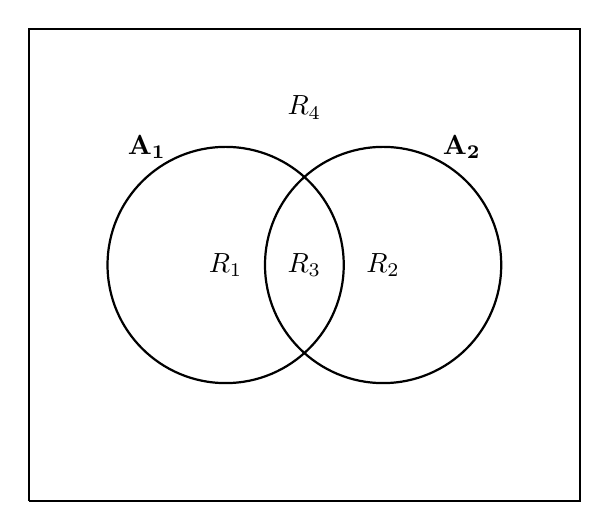
\begin{tikzpicture}
			\draw[thick] (3,4) circle [radius=1.5];
			\draw[thick] (5,4) circle [radius=1.5];
			\draw[thick] (0.5,1)--(0.5,7)--(7.5,7)--(7.5,1)--(0.5,1);
			\node at (2,5.5) {${\bf A_{1}}$};
			\node at (6,5.5) {${\bf A_{2}}$};
			\node at (3,4) {$R_{1}$};
			\node at (5,4) {$R_{2}$};
			\node at (4,4) {$R_{3}$};
			\node at (4,6) {$R_{4}$};
			\end{tikzpicture}	
		\end{center}	
	\end{figure}

\end{document}